% !TEX root = github-tutorial.tex
\section{Adding Content}

On your local machine, create a LaTeX file with the following minimal content in the directory where you cloned the repository.  We assume for the remainder of this tutorial that the file name is \Code{mydocument.tex} but feel free to change the name and adjust actions as necessary.
\begin{FileVerbatim}
\documentclass{article}

\begin{document}
\end{document}
\end{FileVerbatim}

Now before we commit the new file, we may also want to edit the already committed \Code{.gitignore} file to include the build product from running LaTeX on our main file.  Therefore, add a line with the PDF file name of the main LaTeX document to the file \Code{.gitignore} so that it looks like the following.
\begin{FileVerbatim}
...
*.tdo
mydocument.pdf
\end{FileVerbatim}

To do so, you can either use a text editor or this command if you are using bash (use the first command to verify this):
\begin{CodeVerbatim}
$ echo $SHELL
/bin/bash
$ cat >> .gitignore <<EOF
> mydocument.pdf
> EOF
\end{CodeVerbatim}

The sections below show how to add and commit the new file and any edits using the GitHub for Mac application or with the command line.

\subsection{Committing with GitHub for Mac}

\begin{figure}
\centering
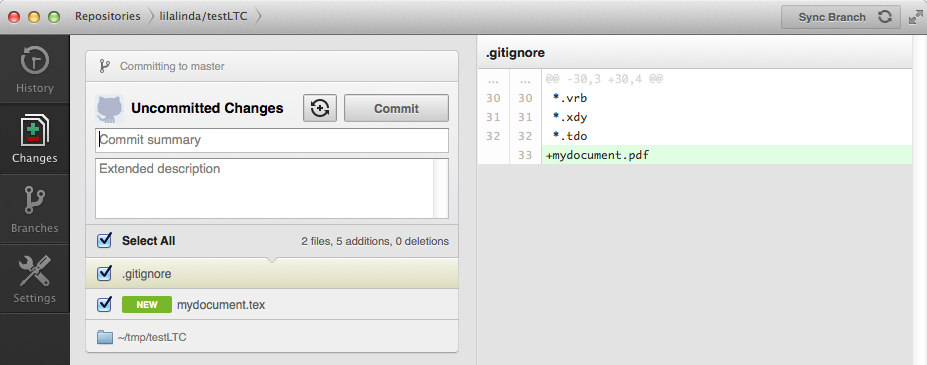
\includegraphics[scale=\myscale]{figures/github-mac-new-file}
\caption{New and edited files with GitHub for Mac} \label{fig:github-mac-new-file}
\end{figure}
If you are using GitHub for Mac, the ``Changes'' tab when inside the repository becomes illuminated when we save the new file and edit the existing one.  Clicking shows a view similar to the one in Figure~\ref{fig:github-mac-new-file}.  

\begin{wrapfigure}{r}{0pt}
\centering
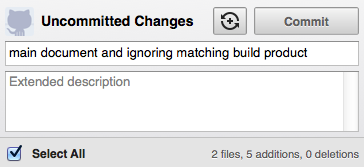
\includegraphics[scale=\myscale]{figures/github-mac-first-commit-msg}
\caption{Commit message in GitHub for Mac} \label{fig:github-mac-first-commit-msg}
\end{wrapfigure}
To commit, provide a meaningful message like ``main document and ignoring matching build product'' as seen in Figure~\ref{fig:github-mac-first-commit-msg} and then click the ``Commit'' button.  After the commit, the application shows Unsynced Commits in the bottom panel, which you can ignore until it is time to sync with GitHub pushing your changes there for your coauthors to enjoy.

\subsection{Committing with the Command Line}

If you are working with the command line, check the status of the repository.
\begin{CodeVerbatim}
$ git status
# On branch master
# Changes not staged for commit:
#   (use "git add <file>..." to update what will be committed)
#   (use "git checkout -- <file>..." to discard changes in working directory)
#
#	modified:   .gitignore
#
# Untracked files:
#   (use "git add <file>..." to include in what will be committed)
#
#	mydocument.tex
no changes added to commit (use "git add" and/or "git commit -a")
\end{CodeVerbatim}

Now add the new file and then commit both using the \Code{-a} switch as seen below.  
\begin{CodeVerbatim}
$ git add mydocument.tex
$ git commit -am "main document and ignoring matching build product"
[master 0893956] main document and ignoring matching build product
 2 files changed, 5 insertions(+)
 create mode 100644 mydocument.tex
\end{CodeVerbatim}

If you check the status after the commit, it will tell you that you are no longer in sync with the server (origin of repository), which you can ignore until it is time to push your changes back to GitHub for your coauthors to enjoy.
\begin{CodeVerbatim}
$ git status
# On branch master
# Your branch is ahead of 'origin/master' by 1 commit.
#   (use "git push" to publish your local commits)
#
nothing to commit, working directory clean
\end{CodeVerbatim}

\section{Sharing Your Work} \label{sec:sharing}

To share your work with your coauthors, you will want to push your local repository at times to the server.  Also, if others are pushing their changes to the server you will want to occasionally pull their changes into your local repository.  The sections below show how to share your work using the GitHub for Mac application or with the command line.

\subsection{Synchronizing with the Server with GitHub for Mac}

In the ``Changes'' panel of the application, click the ``Sync'' button.  This may take a moment as the application is exchanging data with the remote GitHub server.  After a successful synchronization, the icon in the left bar becomes gray scale signaling that there are no lingering edits or commits and your local repository is in sync with the remote repository.

Let us edit the main document to show ongoing work, for example by adding the following line to the LaTeX preamble:
\begin{FileVerbatim}
\usepackage{url} % for typesetting URL's
\end{FileVerbatim}
Once saved, the application shows the uncommitted change in the ``Changes'' panel.  Let us commit with a message such as ``things for the LaTeX preamble'' and then do further edits to the file, for example another package import statement, and save it to disk.
\begin{FileVerbatim}
\usepackage{color}
\end{FileVerbatim}
Even though the ``Sync'' button appears in the ``Unsynced Commits'' panel, clicking it results in a failure message as we have uncommitted changes to the file.  Only when all edits for tracked files are committed will the synchronization work.

\subsection{Synchronizing with the Server with the Command Line}

To upload your latest commits to the GitHub server, you use the \Code{push} command, for example:
\begin{CodeVerbatim}
$ git push
Counting objects: 6, done.
Delta compression using up to 8 threads.
Compressing objects: 100% (4/4), done.
Writing objects: 100% (4/4), 442 bytes | 0 bytes/s, done.
Total 4 (delta 1), reused 0 (delta 0)
To git@github.com:lilalinda/testLTC.git
   387b684..672c28b  master -> master
\end{CodeVerbatim}

If you are working with git branches, you may have to specify the branch with this command but that is for more complicated scenarios (often not needed for writing projects).  

The opposite command to obtain changes from the server, as a coauthor had pushed some edits to the text, use the \Code{pull} command, for example:
\begin{CodeVerbatim}
$ git pull
remote: Counting objects: 5, done.
remote: Compressing objects: 100% (1/1), done.
remote: Total 3 (delta 2), reused 3 (delta 2)
Unpacking objects: 100% (3/3), done.
From github.com:lilalinda/testLTC
   498aac2..70beabe  master     -> origin/master
Updating 498aac2..70beabe
Fast-forward
 mydocument.tex | 1 +
 1 file changed, 1 insertion(+)
\end{CodeVerbatim}

As long as there are no conflicts that git cannot resolve, this command merges any remote changes with your working copy.  You should make sure to have no lingering changes waiting to be committed when you pull from the remote repository.  The man page for the \Code{git-pull} command says:
\begin{quote}
If any of the remote changes overlap with local uncommitted changes, the merge will be automatically cancelled and the work tree untouched. It is generally best to get any local changes in working order before pulling or stash them away with \Code{git-stash}.
\end{quote}
